%% This is file `elsarticle-template-3-num.tex',
%%
%% Copyright 2009 Elsevier Ltd
%%
%% This file is part of the 'Elsarticle Bundle'.
%% ---------------------------------------------
%%
%% It may be distributed under the conditions of the LaTeX Project Public
%% License, either version 1.2 of this license or (at your option) any
%% later version.  The latest version of this license is in
%%    http://www.latex-project.org/lppl.txt
%% and version 1.2 or later is part of all distributions of LaTeX
%% version 1999/12/01 or later.
%%
%% The list of all files belonging to the 'Elsarticle Bundle' is
%% given in the file `manifest.txt'.
%%
%% Template article for Elsevier's document class `elsarticle'
%% with numbered style bibliographic references
%%
%% $Id: elsarticle-template-3-num.tex 165 2009-10-08 07:58:10Z rishi $
%% $URL: http://lenova.river-valley.com/svn/elsbst/trunk/elsarticle-template-3-num.tex $
%%

\documentclass[final,times,5p]{elsarticle}

%% Use the option review to obtain double line spacing
%% \documentclass[preprint,review,12pt]{elsarticle}

%% Use the options 1p,twocolumn; 3p; 3p,twocolumn; 5p; or 5p,twocolumn
%% for a journal layout:
%% \documentclass[final,1p,times]{elsarticle}
%% \documentclass[final,1p,times,twocolumn]{elsarticle}
%% \documentclass[final,3p,times]{elsarticle}
%% \documentclass[final,3p,times,twocolumn]{elsarticle}
%% \documentclass[final,5p,times]{elsarticle}
%% \documentclass[final,5p,times,twocolumn]{elsarticle}

%% PACKAGES

%% if you use PostScript figures in your article
%% use the graphics package for simple commands
%% \usepackage{graphics}
%% or use the graphicx package for more complicated commands
\usepackage{graphicx}
%% or use the epsfig package if you prefer to use the old commands
%% \usepackage{epsfig}

%% The amssymb package provides various useful mathematical symbols
\usepackage{amssymb}
%% The amsthm package provides extended theorem environments
%% \usepackage{amsthm}

%% The numcompress package shorten the last page in references.
%% `nodots' option removes dots from firstnames in references.
%% `nocompress' option prevent shortening of last page as
%% by default it will shorten.

\usepackage[nodots]{numcompress}
%% The lineno packages adds line numbers. Start line numbering with
%% \begin{linenumbers}, end it with \end{linenumbers}. Or switch it on
%% for the whole article with \linenumbers after \end{frontmatter}.
%% \usepackage{lineno}

%% natbib.sty is loaded by default. However, natbib options can be
%% provided with \biboptions{...} command. Following options are
%% valid:

%%   round  -  round parentheses are used (default)
%%   square -  square brackets are used   [option]
%%   curly  -  curly braces are used      {option}
%%   angle  -  angle brackets are used    <option>
%%   semicolon  -  multiple citations separated by semi-colon
%%   colon  - same as semicolon, an earlier confusion
%%   comma  -  separated by comma
%%   numbers-  selects numerical citations
%%   super  -  numerical citations as superscripts
%%   sort   -  sorts multiple citations according to order in ref. list
%%   sort&compress   -  like sort, but also compresses numerical citations
%%   compress - compresses without sorting

\usepackage{lineno}

%\usepackage{fleqn}
\usepackage{tikz}
\usepackage{pgfplots}
\usepackage{booktabs}
\usepackage{multirow}
\usepackage{amsmath}
\usepackage{nomencl}
\usepackage{framed} % Framing content
\usepackage{multicol} % Multiple columns environment
\usepackage{float}
\usepackage{rotating}
\usepackage{float}
\usepackage[pdftex,bookmarks=true]{hyperref}
\hypersetup{ 
    colorlinks,% 
    citecolor=black,% 
    filecolor=black,% 
    linkcolor=black,% 
    urlcolor=black 
} 

\biboptions{square,sort&compress}

%% Contraction of references
\makeatletter
\def\NAT@spacechar{}
\makeatother

\renewcommand*\nompreamble{\begin{multicols}{2}}
\renewcommand*\nompostamble{\end{multicols}}

\RequirePackage{ifthen}

\renewcommand{\nomgroup}[1]{%
\ifthenelse{\equal{#1}{0}}{\item[\emph{Symbols}]}{
\ifthenelse{\equal{#1}{S}}{\item[\emph{Subscripts}]}{}}
\ifthenelse{\equal{#1}{P}}{\item[\emph{Superscripts}]}{
\ifthenelse{\equal{#1}{A}}{\item[\emph{Abbreviations}]}{}}
\ifthenelse{\equal{#1}{G}}{\item[\emph{Greek letters}]}{
\ifthenelse{\equal{#1}{O}}{\item[\emph{Others}]}}
}

\makeindex
\makenomenclature

\journal{Energy}

% Make the footnote space disappear for the first page (preprint and journal)
 
%\makeatletter
%\def\ps@pprintTitle{%
% \let\@oddhead\@empty
% \let\@evenhead\@empty
% \def\@oddfoot{}%
% \let\@evenfoot\@oddfoot}
%\makeatother

\begin{document}

\begin{frontmatter}

\title{Thermodynamic assessment of the Kalina Split Cycle}

\author[]{Tuong-Van Nguyen\corref{cor}} \cortext[cor]{Principal corresponding author. Tel.: +45 4525 4129} \ead{tungu@mek.dtu.dk}
\author[]{Thomas Knudsen} 
\author[]{Ulrik Larsen} 
\author[]{Brian Elmegaard} 
\author[]{Fredrik Haglind} 

\address{Section of Thermal Energy, Department of Mechanical Engineering, Technical University of Denmark,\\ Building 403, Nils Koppels All\'{e}, 2800 Kongens Lyngby, Denmark}

\begin{abstract}

The Kalina Split Cycle is a thermodynamic process for converting thermal energy into electrical power, (i) using the ammonia-water mixture as working fluid, like a conventional Kalina Cycle, and (ii) with a varying ammonia concentration during the heat extraction. This second feature results in an improved match between the heat source and working fluid temperature profiles, decreasing the entropy generation in the heat recovery system.  
The present work compares the thermodynamic performance of this power cycle with other configurations of the Kalina process, and investigates the impact of varying operating conditions. The results indicate that the Kalina Split Cycle with reheat presents an exergetic efficiency higher by 2.8\% points than a reference Kalina cycle with reheat, and by 4.3\% points without. The cycle performance is highly sensitive to its boundary conditions, varying by 9\% for a temperature variation of 30$^{\circ}$C for the cold reservoir and 100$^{\circ}$C for the stack. This analysis also pinpoints the large irreversibilities in the low-pressure turbine and condenser, which have an efficiency defect of 9.5-13\% and 7.2-13.7\%, respectively, and indicates a reduction of the exergy destruction by about 23\% in the heat recovery system. 

\end{abstract}

\begin{keyword}
Kalina Split Cycle \sep Energy analysis \sep Exergy assessment \sep Waste Heat Recovery 
\end{keyword}

\end{frontmatter}

%
%% Start line numbering here if you want
%%
\linenumbers

%% Main Text

%%%%%%%%% SECTION: INTRODUCTION %%%%%%%%%

\section{Introduction}
\label{sec:introduction}
	
%%%%%%%%% NOMENCLATURE %%%%%%%%%

\begin{table*}[!ht]
  \begin{framed}
  \footnotesize
    \printnomenclature
  \end{framed}
\end{table*}


Waste heat recovery (WHR) systems are able to generate mechanical power and electricity without any fuel input and associated CO$_2$ emissions. Hence, with rising fuel prices and increased environmental awareness, motivation is growing for integrating these systems to improve the energy efficiency of various processes. An example is a WHR system for large marine engines in the present study. Organic Rankine cycles (ORC) and Kalina cycles are among the most frequently proposed alternatives to steam Rankine cycle WHR systems. At the scale of application studied in the present work, i.e. a net power output of 1-5 MW, both power cycles may be viable \cite{Tchanche20113963,Jonsson2001c}. Bombarda et al. \cite{Bombarda2010b} compared the two processes for a heat source temperature level of 346$^\circ$C and found that both cycles, when optimised, produced almost equal net power outputs. While the present study does not directly compare the ORC with the Kalina cycle, this work is based on the boundary conditions used in the work of Bombarda et al. \cite{Bombarda2010b}, in order to make comparisons about the power cycle performance for the same application.

Energy can neither be created nor destroyed, and an energy analysis illustrates the energy transformations and flows throughout the system under study. On the opposite, exergy is not conserved in real processes, illustrating therefore the locations, causes and magnitudes of the thermodynamic irreversibilities taking place \cite{BejanAdrian;TsatsaronisGeorge;Moran1996,Bejan2006}. Exergy destruction also accounts for the additional exergetic fuel required because of the system imperfections \cite{Wall1988,Kotas1980,Kotas1980a,Kotas1995}. A few studies on the thermodynamic performance of the Kalina cycle exist. 

The present paper presents and evaluates a novel power generation cycle, called the Kalina Split Cycle. This process is also based on the ammonia-water mixture as working fluid, like the conventional Kalina Cycle, but is characterised by a varying ammonia concentration in the heat recovery system. This results in a smaller entropy generation in the heat transfer process, and potentially in a higher exergetic efficiency of the complete power cycle. This concept was briefly mentioned in the work of Kalina, and a system analysis was previously conducted by the same authors to identify the governing mechanisms of this process. The literature appears to contain little, if none, on the thermodynamic performance of such cycle, and this study aims at closing this gap, following these three objectives:

\begin{itemize}

	\item estimation of the cycle potential, in terms of energy and exergy efficiencies, compared to a conventional Kalina cycle, with and without reheat;
	\item analysis of the plant inefficiencies and of the exergy destruction trends;
	\item evaluation of the impact of the boundary conditions (heat source and cold reservoir temperatures) on the performance of this system;

\end{itemize}

Section \ref{sec:system_description} presents the design of the Kalina Split Cycle system and the methods used in this work are reported in Section \ref{sec:methods}. The results are presented in Section \ref{sec:results} and are criticised further in Section \ref{sec:discussion}. Concluding remarks are outlined in Section \ref{sec:conclusion}.

\nomenclature[A]{ASPEN}{Advanced System for Process Engineering}
\nomenclature[A]{WHR}{waste heat recovery}
\nomenclature[A]{ORC}{Organic Rankine Cycle}
\nomenclature[A]{SC}{Split Cycle}
\nomenclature[A]{SUP}{superheated state}
\nomenclature[A]{SUB}{sub-cooled state}

%%%%%%%%% SECTION: SYSTEM DESCRIPTION %%%%%%%%%

\section{System description}
\label{sec:system_description} 
The reference Kalina process layout and the process conditions used throughout were the same as those presented in the work of Bombarda et al. \cite{Bombarda2010b}. Both the reference cycle and the Split-cycle were evaluated with and without using reheat in the turbine, in order to determine the influence of this technique on the processes. 

In the following, the solution concentration running through the turbine is referred to as the \emph{working solution}, and the terms \emph{lean} and \emph{rich} refer to a low and a high concentration of ammonia in the solution, respectively.

\subsection{Reference Kalina cycle}
\label{sec:kalina_cycle}
\begin{figure*}[htbp]
\centering
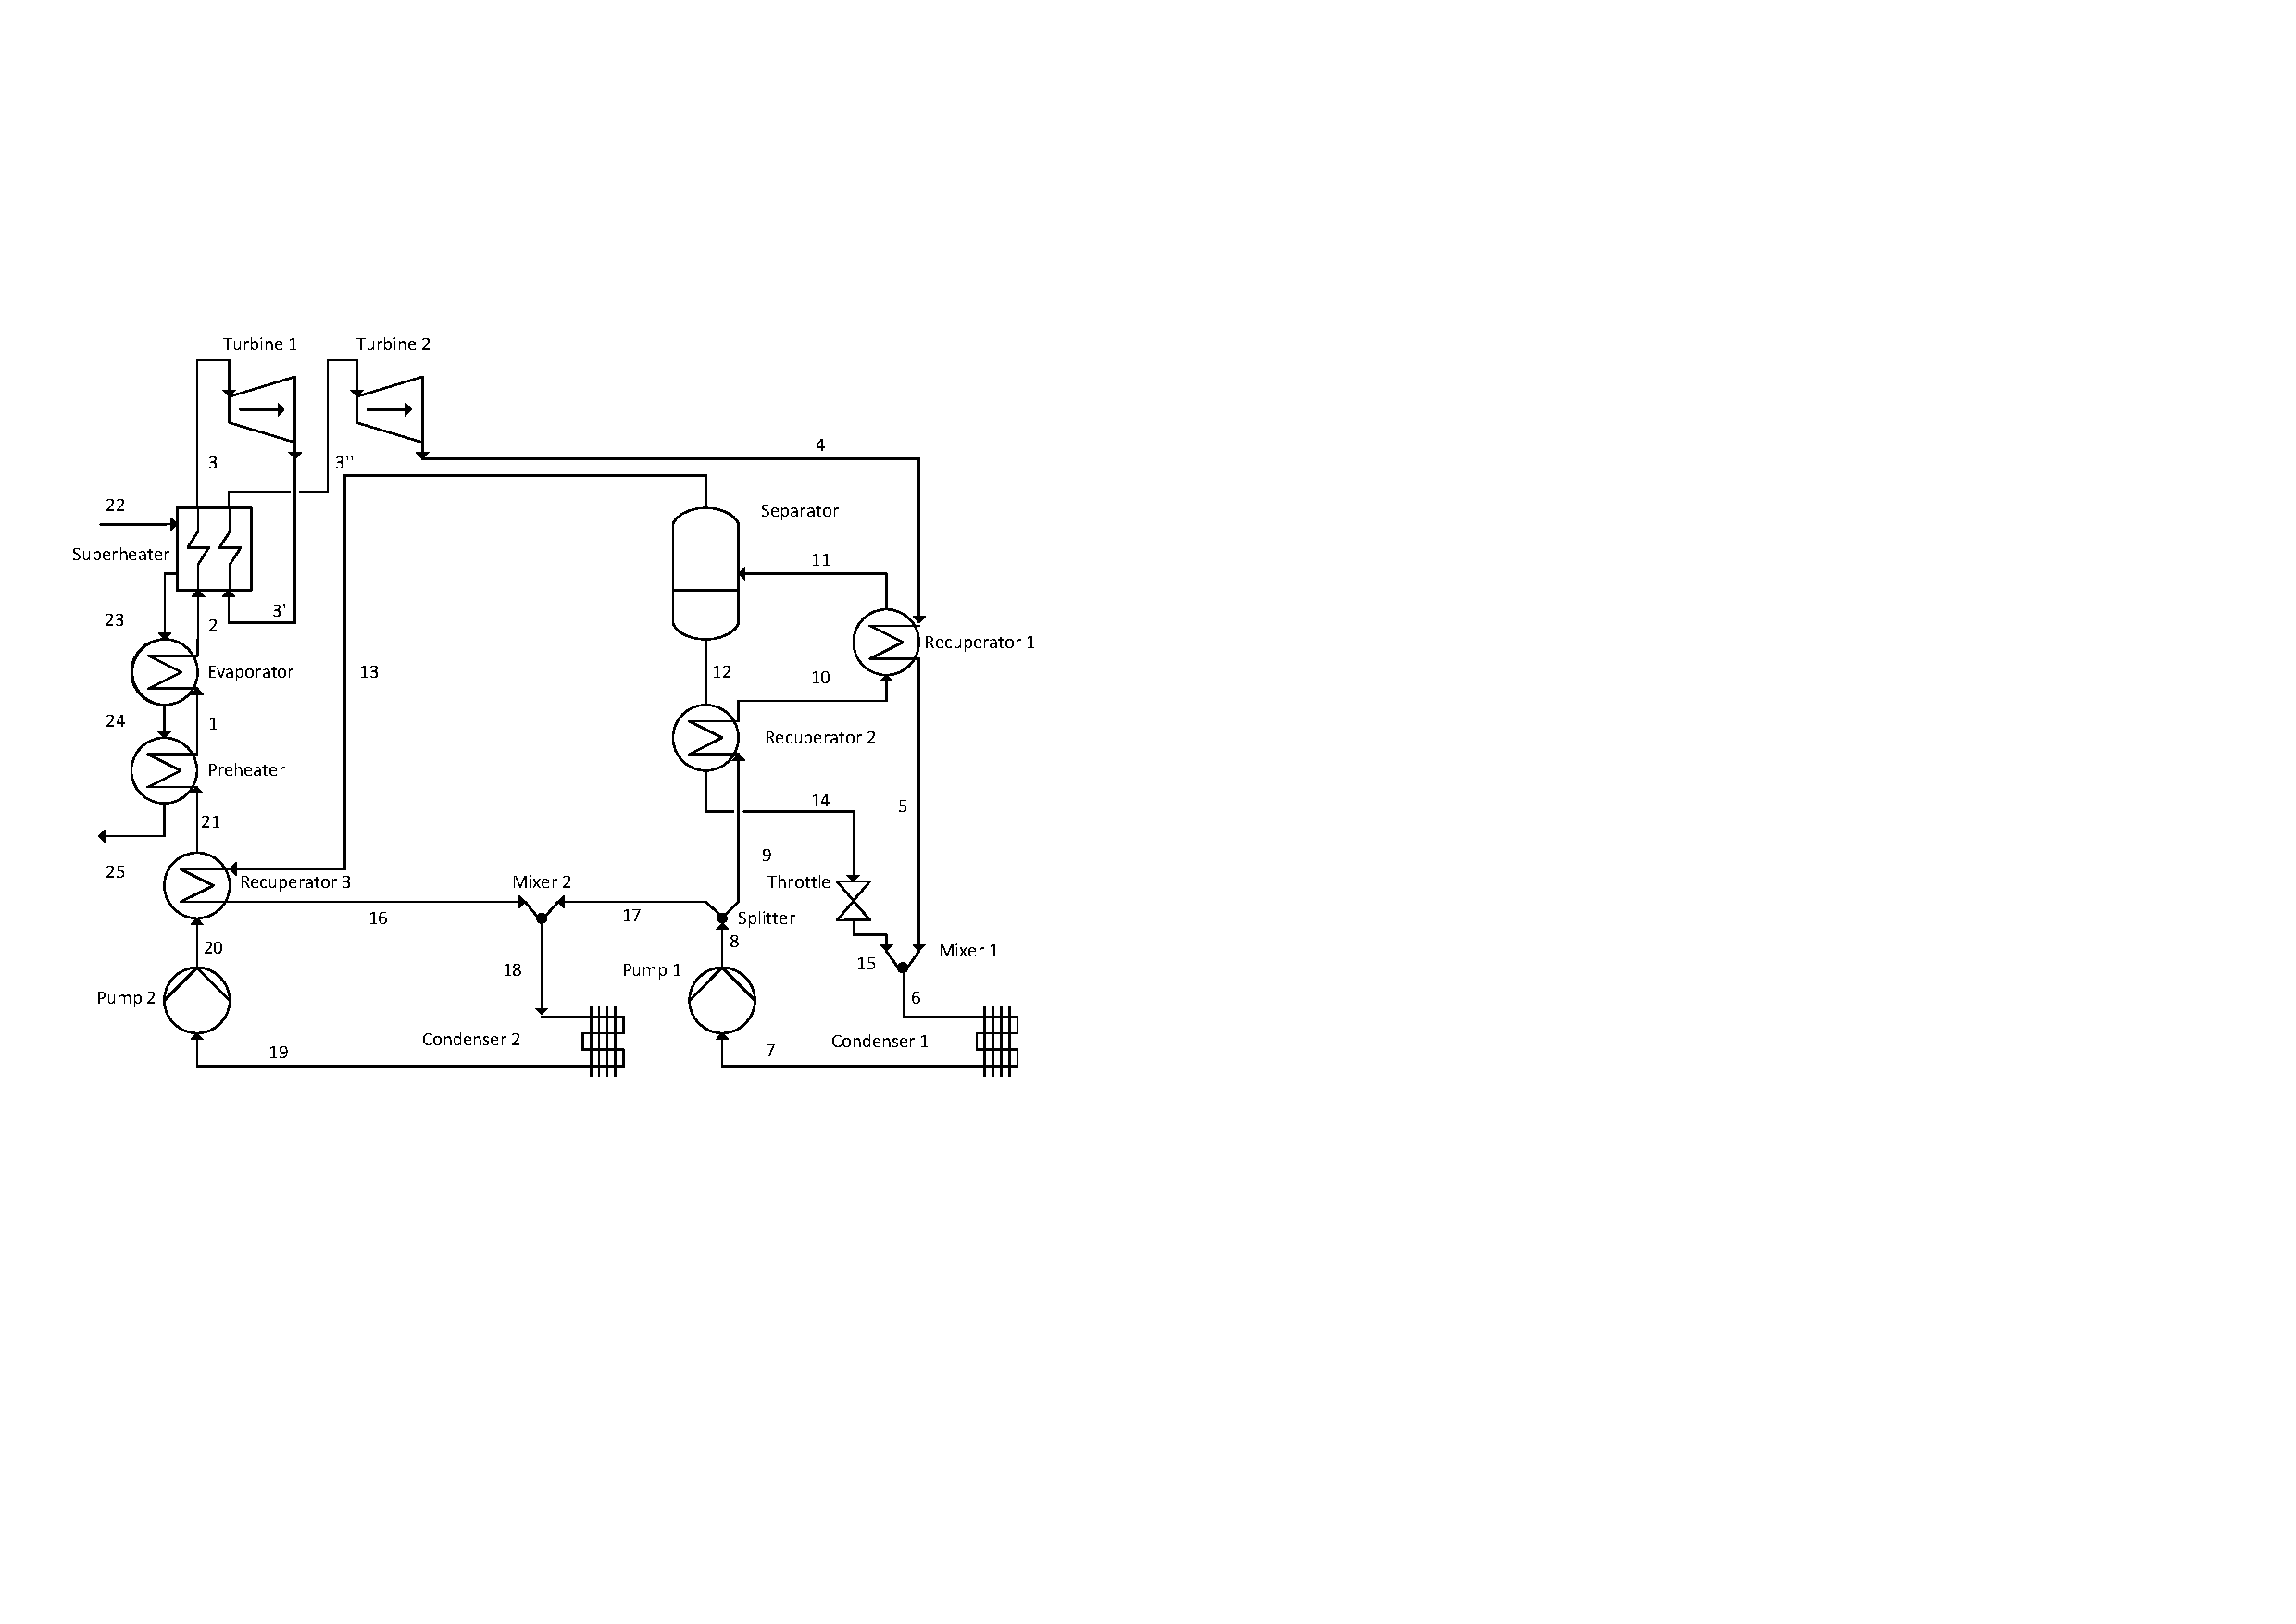
\includegraphics[width=0.9\linewidth]{Drawing_Kalina_Baseline.pdf}
\caption{Sketch of the Kalina reference process with reheat}
\label{fig:kalina_cycle}
\end{figure*}

Figure \ref{fig:kalina_cycle} illustrates the flow diagram of the reference Kalina process with reheat. Starting from (21) to (1), the preheated working fluid is evaporated and superheated in the boiler before it enters the turbine (3). In the process layout that includes the reheat technique, the outlet stream from the turbine (3') is heated in the boiler before entering (3'') a second turbine. When reheat is not included in the process, stream (3) runs directly from the turbine outlet (4) to Recuperator 1. From the stream (4) heat is transferred to the stream (10) in Recuperator 1. The stream (5) is then mixed with an ammonia lean stream from the separator (15) to form a leaner solution. This solution is condensed (7) and after being pumped to an intermediate pressure level, the stream (8) is divided into two streams (9) and (17). The stream (9) is heated in Recuperator 2 and in Recuperator 1 to a partially evaporated state. It then enters the separator which separates the stream into a lean liquid (12) and a very rich vapour (13). Heat from stream (13) is used to preheat stream (20) in Recuperator 3, and the stream (16) is then mixed with a leaner solution (17) to form the working solution (18). This stream is finally condensed and pumped to the boiler pressure. 

\subsection{Kalina Split-cycle}
\label{sec:split_cycle}
\begin{figure*}[htbp]
\centering
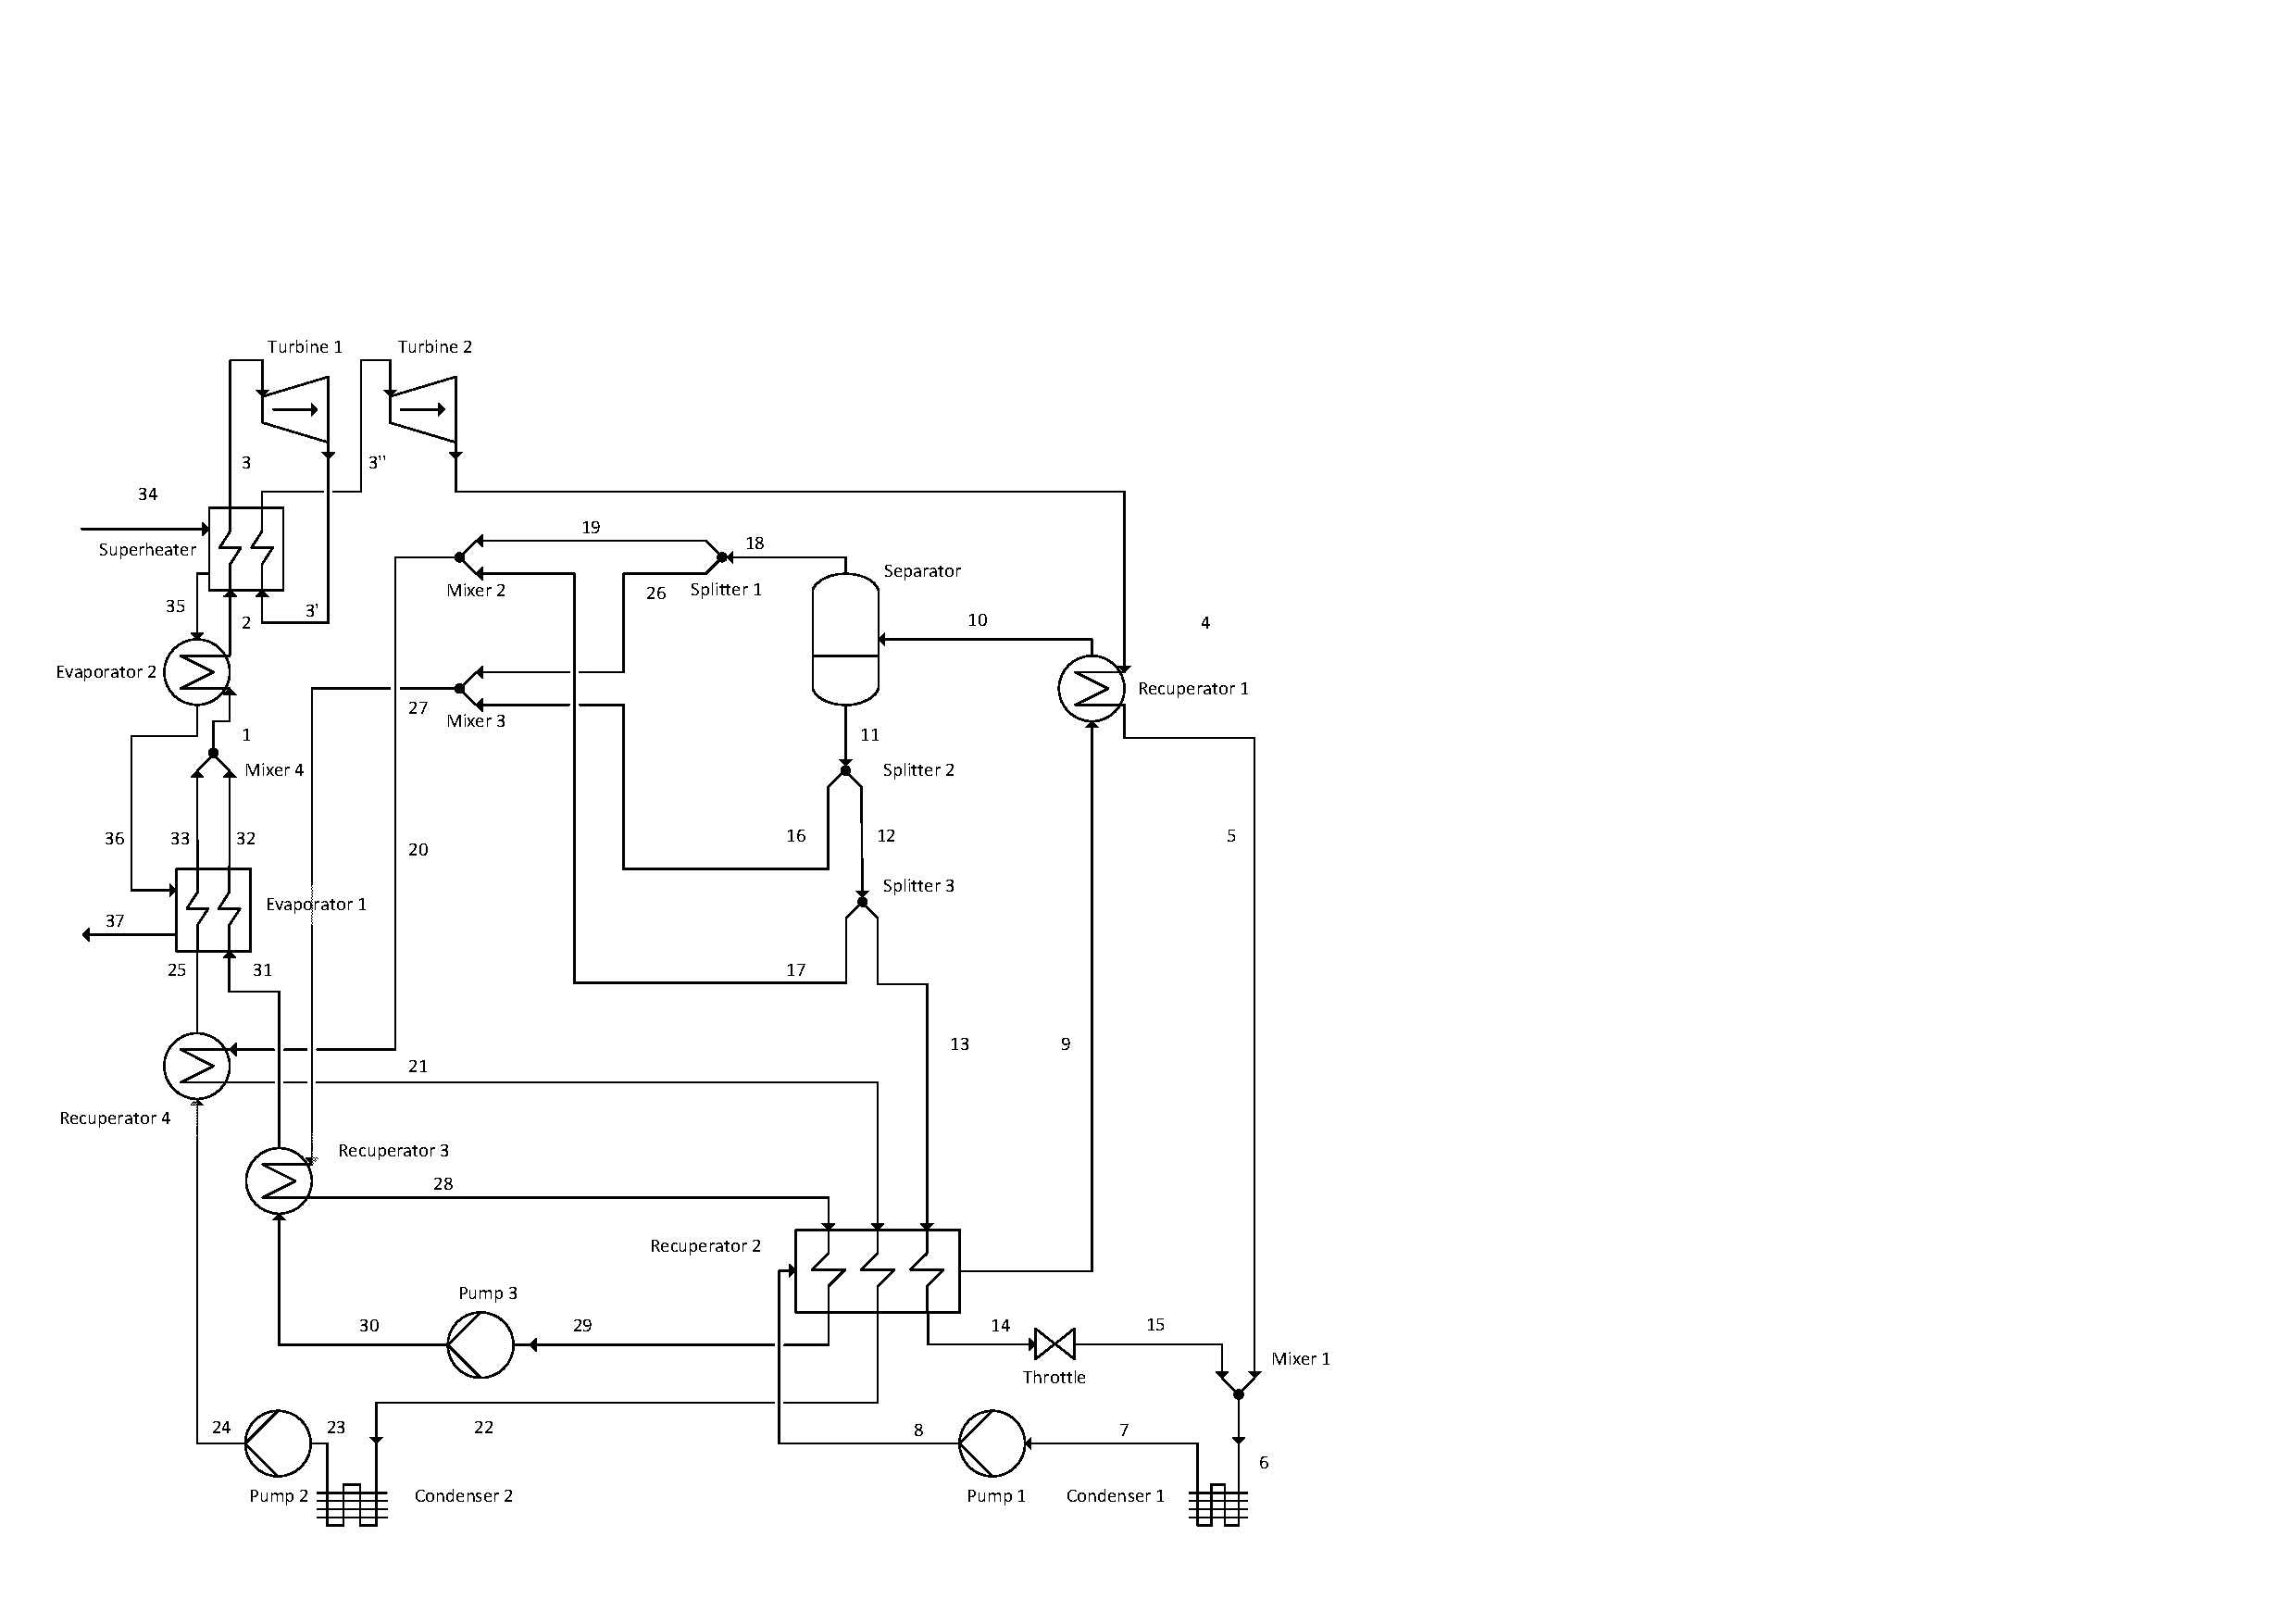
\includegraphics[width=1.0\linewidth]{Drawing_Kalina_Split.pdf}
\caption{Sketch of the Kalina Split-cycle process}
\label{fig:split_cycle}
\end{figure*}

Figure \ref{fig:split_cycle} illustrates the flow diagram of the Split-cycle process. To maintain focus on the special split stream boiler, the Split-cycle configuration modelled in this work was designed to have a minimum number of components needed for evaluating the concept. Hence, the SC presented here is based on the same principles as the reference Kalina cycle, with some important differences. 

Two streams of different ammonia concentration enter the boiler, a rich stream (25) and a lean stream (31). Before being mixed (Mixer 4), the rich stream is fully evaporated, and the lean stream is heated to the bubble point state. The aim of this arrangement is to lower the temperatures in the overall process going from liquid (25,31) to vapour (2). To be able to produce these two streams with the desired concentrations and mass flow rates, an additional mixing subsystem, consisting of three splitters and two mixers, is also needed. 

The gradient of the evaporation temperature curve can to some degree be adjusted to the temperature profile of the heat source by selecting the optimal composition of each of the two streams, as illustrated in Fig. \ref{fig:theory}. The line from (25,31) to the point ($T_{r,b}$)\nomenclature[S]{r}{rich ammonia concentration} \nomenclature[S]{b}{bubble point}represents the preheat stage. From here to points (1), (2) and (3) the fully drawn line represents the heat transfer when using the Split-cycle configuration. The upper dashed line represents how the heat transfer would be if the two streams were combined into a single stream. The point ($T_{b}$) signifies the bubble point of the combined stream, and it is clear that the temperature difference at the pinch point is much smaller and possibly violated in this case. The lower dashed line from ($T_{r,b}$) through (2a) to (2), shows how the heat transfer would occur if only the rich stream concentration was used. Evaporation would take place at lower temperatures possibly leading to a lower thermal efficiency. 



\begin{figure*}[htpb]
\centering
\begin{tikzpicture}[scale=0.9]

\begin{axis}[xlabel={Accumulated heat transfer},
	ylabel={Temperature},
	axis lines*=left,
	legend pos=outer north east,
	no markers,
	xticklabels={,,},
	yticklabels={,,}
	]

\addplot [style=thick] table[x index=0,y index=1,col sep=space] {theory.data}; %split
\addplot table[x index=0,y index=1,col sep=space] {theoryHeatSource.data}; %heat source
\addplot [style=dashed] table[x index=0,y index=1,col sep=space] {theoryRich.data}; %rich alone
\addplot [style=dashed] table[x index=0,y index=1,col sep=space] {theoryComp.data}; %composite

\node[] at (40,1) {$25,31$}; 
\node[] at (100,22) {$T_{r,b}$};
\node[] at (50,50) {$T_{b}$};
\node[] at (200,60) {$1$};
\node[] at (300,70) {$2$};
\node[] at (270,45) {$2a$};
\node[] at (400,92) {$3$};
\node[] at (0,25) {$37$};
\node[] at (400,112) {$34$};

\end{axis}
\end{tikzpicture}

\caption{Sketch of T-Q diagram of the heat recovery system to explain the Split-cycle}
\label{fig:theory}
\end{figure*}






Kalina argued \cite{Kalina1986a} that the state of the rich stream at point (33) (Fig. \ref{fig:split_cycle}) should ideally be at the dew point and that the lean stream at point (32) should be at the bubble point, before the mixing of the two streams. The two streams should also have similar temperatures and pressures in order to minimise the entropy generation in this section of the boiler. We decided to adopt these constraints without further analysis to focus on the full process analysis. However, an entropy generation analysis is planned for future work to verify this claim. In the following, these conditions are referred to as the SC boiler constraints. 

A direct consequence of the SC boiler constraints is that, once the ammonia concentration of one of the streams, (25) or (31), has been chosen, the concentration of the other is fixed in order to satisfy the equilibrium conditions. Additionally, when the boiler pressure and the concentration in one stream are chosen, the temperature of the working fluid streams out of evaporator 1 is fixed. Both are illustrated in the example shown in Fig. \ref{fig:bubbleDew}. As shown, the mixing temperature decreases and the lean stream concentration increases, as the rich stream concentration increases. 



\begin{figure}[htpb]
\centering
\begin{tikzpicture}[scale=0.9]

\begin{axis}[xlabel={Rich stream ammonia concentration},
	%xmin=0.75, xmax=1.0,
	ymin=0.2,
	axis x line*=bottom,
	axis y line*=left,
	ylabel={Lean stream ammonia concentration},
	ylabel near ticks,
	legend style={legend pos=south west,font=\small, draw=none} ,
	]

\addplot [mark=triangle*, mark options={fill=black}] table[x index=0,y index=1,col sep=space] {data/bubbleDewPoints.txt};
\addlegendentry{Concentration}

\end{axis}

\begin{axis}[xlabel={},
	%xmin=0.75, xmax=1.0,
	ymin=100,
	axis x line*=bottom,
	hide x axis,
	axis y line*=right,
	ylabel={Mixing temperature ($^\circ$C)},
	ylabel near ticks,
	legend style={legend pos=south east,font=\small, draw=none} ,
	]

\addplot table[x index=0,y index=2,col sep=space] {data/bubbleDewPoints.txt};
\addlegendentry{Temperature}

\end{axis}
\end{tikzpicture}

\caption{Equilibrium conditions for Evaporator 1 outlet}
\label{fig:bubbleDew}
\end{figure}

\section{Methods}
\label{sec:methods}

	\subsection{Process modelling, simulation and validation}

		\subsubsection{Modelling}

		\subsubsection{Simulation}
	
		\subsubsection{Validation}
			
	\subsection{Energy analysis}
	\label{subsec:energy_analysis}
		
	\emph{Energy} may be stored, transformed from one form to another and transferred between systems, but, as stated by the 1st law of thermodynamics, energy can neither be created nor destroyed. In open systems, energy can be transferred in or out of the system under study by streams of matter, heat and work. Neglecting the kinetic and potential energies, the energy rate balance at steady state is:
	
	\begin{equation}
	0=\sum_k \dot{Q}_{k}-\dot{W}_{cv} + \sum \dot{m}_{in} h_{in} - \sum \dot{m}_{out} h_{out}
	\end{equation}
	
	where $\dot{Q}_{k}$ and $\dot{W}_{cv}$ the time rates of energy transfer by heat and work ($\dot{Q}\ge0$ indicates heat transfer to the system, $\dot{W}\ge0$ work done by the system). The subscripts $in$ and $out$ denote the inlet and outlet of the system, $k$ the boundary of the component of interest and $cv$ the control volume. $h$ is the specific enthalpy of the stream under consideration, and can be defined as the change in enthalpy observed when it is brought from its temperature and pressure to the reference conditions, and is decomposed into the reference elements in standard state. 
	
	\nomenclature[0]{h}{specific total enthalpy (mass), J/kg}
	\nomenclature[S]{k}{component}
	\nomenclature[S]{cv}{control volume}
	\nomenclature[S]{in}{inlet}
	\nomenclature[S]{out}{outlet}
	
	The enthalpy change due to temperature and pressure variations is called the specific physical enthalpy $h^{ph}$ and depends on the reference state, fixed in this work to the environmental conditions $T_0$ and $p_0$. The enthalpy change due to chemical deviations with the environment is called the chemical enthalpy $h^{ch}$ and depends on the choice of the reference species and reaction. The reference environment proposed by Szargut is considered in this work. The chemical enthalpy is therefore equal to the enthalpy of devaluation $h_{dev}$ \cite{Kotas1995}, which can be interpreted as the energy released from a given substance interacting with common chemical species present in the environment \cite{Szargut1988}. 
	
	\nomenclature[0]{$h$}{specific enthalpy (mass), J/kg}
	\nomenclature[0]{$h_{dev}$}{specific enthalpy of devaluation (mass), J/kg}	

	The energy balance for the Kalina Split Cycle can be expressed as: 

	\begin{equation}
	 \dot{Q}_{heat}=\dot{W}+\dot{Q}_{cool}
	\end{equation}	

	where $\dot{Q}_{heat}$ is the energy recovered as heat from the waste heat source, $\dot{W}$ the electric power delivered by the plant, and $\dot{Q}_{cool}$ the energy losses due to heat rejection to the environment with the cooling water.
	
	The energy efficiency, or thermal efficiency $\eta_{th}$, is therefore defined as:
	
	\begin{equation}
		\eta_{th} = \frac{\dot{W}}{\dot{Q}_{heat}} 
	\end{equation}	

	The thermal efficiency is limited by the cold and hot reservoir temperatures $T_{cold}$ and $T_{hot}$, and this upper bound is given by the Carnot efficiency $\eta_{carnot}$:
	
	\begin{equation}
		\eta_{carnot} = 1-\frac{T_{cold}}{T_{hot}} 
	\end{equation}
	
	\subsection{Exergy analysis}
	\label{subsec:exergy_analysis}

	\subsubsection{Exergetic accounting and components}
	
	\emph{Exergy} may be defined as the `maximum theoretical useful work (shaft work or electrical work) as the system is brought into complete thermodynamic equilibrium with the thermodynamic environment while the system interacts with this environment only'. Exergy is not conserved in real processes as it is destroyed because of internal irreversibilities. The exergy balance is expressed as \cite{BejanAdrian;TsatsaronisGeorge;Moran1996}: 

	\begin{align}
		\dot{E}_d&=\sum \dot{E}_{in} - \sum \dot{E}_{out} \nonumber\\
					  &=\sum_k \left (1-\frac{T_0}{T_k} \right ) \dot{Q}_j-\dot{W}_{cv}+\sum \dot{m}_{in} e_{in} - \sum \dot{m}_{out} e_{out}
	\end{align}

	where $\dot{E}_d$, $\dot{E}_{in}$ and $\dot{E}_{out}$ are the exergy destruction, inflows and outflows, respectively. $e$ is the specific exergy of a material stream, $T_0$ and $T_k$ are the environmental and instantaneous temperatures. The exergy destruction rate can be calculated from the Gouy-Stodola theorem, which is, on a time rate form, expressed as \cite{Bejan2006}:

	\nomenclature[0]{$e$}{specific exergy (mass), J/kg}
	\nomenclature[0]{$\dot{S}$}{entropy rate, W/K}
	\nomenclature[S]{gen}{generation}
	\nomenclature[0]{$p$}{pressure, Pa}
	\nomenclature[0]{$\dot{E}$}{exergy rate, W}
	\nomenclature[S]{d}{destruction} 
	\nomenclature[S]{l}{loss} 
	\nomenclature[S]{0}{dead state} 
	\nomenclature[P]{$^{*}$}{relative}	
	\nomenclature[0]{$T$}{temperature, K}
		
	\begin{equation}
		\dot{E}_d=T_0\dot{S}_{gen}
	\end{equation}
	
	where $\dot{S}_{gen}$ is the entropy generation rate.

	Exergy destruction is also called `internal exergy losses', as they are related to the irreversibilities taking place within the system, i.e. \emph{inside} the control volume under study. This corresponds, for instance, to the inefficiencies of the turbines and pumps. The term exergy loss, also called `external exergy losses' and written $\dot{E}_l$, refers to the exergy released to the environment without any practical use, i.e. \emph{outside} the control volume under study, such as the exergy gain of the cooling water \cite{Szargut1998,Kotas1995,BejanAdrian;TsatsaronisGeorge;Moran1996}. 

	In the absence of nuclear, magnetic and electrical interactions, the exergy associated with a stream of matter is a function of its physical $e^{ph}$, chemical $e^{ch}$, kinetic $e^{kn}$ and potential $e^{pt}$ components \cite{BejanAdrian;TsatsaronisGeorge;Moran1996}. Therefore, on a unit mass basis, the specific exergy of a material stream is expressed as:

	\nomenclature[P]{ph}{physical} 
	\nomenclature[P]{ch}{chemical} 
	\nomenclature[P]{kn}{kinetic} 
	\nomenclature[P]{pt}{potential} 
	\nomenclature[0]{$\bar{e}$}{specific exergy (molar), J/mol} 
	\nomenclature[0]{$y$}{component/sub-system exergy ratio} 
		
	\begin{equation}
		e=e^{ph}+e^{ch}+e^{kn}+e^{pt}
	\end{equation}

	Physical exergy accounts for temperature and pressure differences from the environmental state and is defined as:  
		
	\begin{equation}
		e^{ph}=(h-h_0)-T_0(s-s_0) 
	\end{equation}
	
	where $s$ is the specific entropy of a stream of matter per unit-of-mass, respectively. 

	Chemical exergy accounts for deviations in chemical composition from reference substances present in the environment. In this work, chemical exergy is calculated based on the concept of \emph{standard chemical exergy} discussed by Moran and Shapiro \cite{Moran2007}. The specific chemical exergy of real chemical compounds is determined using the reference environment defined by Szargut \cite{Szargut1988,Szargut1989,Morris1986}.

	\nomenclature[0]{$s$}{specific entropy (mass), J/(kg$\cdot$K)}
	\nomenclature[S]{j}{stream}
	
	The specific chemical exergy of a given mixture $\bar{e}^{ch}_{mix}$, on a molar basis, is expressed as \cite{Sato2004}:

	\begin{align}
		\bar{e}^{ch}_{mix}=&\underbrace{\sum_i \bar{x}_i \bar{e}^{ch}_{i,mix}}_{I} \nonumber\\
		=&\underbrace{\sum_i \bar{x}_i \bar{e}^{ch}_{i,0}}_{II}+\underbrace{\left(\sum_i \bar{x}_i \left(h_{i,mix}-h_{i,0}\right)\right)-T_0\left(\sum_i \bar{x}_i \left(s_{i,mix}-s_{i,0}\right)\right)}_{III}
	\end{align}

	where the molar fraction, the chemical compound and the mixture are denoted by $\bar{x}$, $i$ and $mix$, respectively. The specific molar exergy of a given chemical compound is written $\bar{e}^{ch}_{i,mix}$ when it is in the mixture and $\bar{e}^{ch}_{i,0}$ when it is in a pure component state. The term $I$ illustrates the chemical exergy of each individual chemical compound in the mixture, the term $II$ the chemical exergy of these compounds in an unmixed form and the term $III$ the reduction in chemical exergy due to mixing effects.  
	
	\nomenclature[S]{i}{chemical compound}
	\nomenclature[S]{mix}{mixture}

	Kinetic and potential contributions are not considered in this work. Exergy transported with work is equal to its energy and depends on the system and environmental temperatures when it is transferred with heat:

	\begin{align} 
		\dot{E}^w=&\dot{W}_{cv}\\
		\dot{E}^q=&\left(1-\frac{T_0}{T_j}\right)\dot{Q}_{j}
	\end{align}

	\nomenclature[P]{w}{work}
	\nomenclature[P]{q}{heat}

	The tracing of the energy and exergy flows provides information on the system transformations and inefficiencies: several performance parameters were developed to illustrate the possibilities for improvements and illustrate the components on which improvement efforts should focus \cite{BejanAdrian;TsatsaronisGeorge;Moran1996,Kotas1980,Kotas1980a,Kotas1995}. 

	\begin{itemize}	
		\item The exergy destruction ratio $y_{d}^{*}$ is defined as the ratio of the exergy destruction rate $\dot{E}_{d,k}$ within a specific component $k$ to the total exergy destruction rate in the overall system $\dot{E}_{d}$:  
	\begin{equation} y_{d}^{*}=\frac{\dot{E}_{d,k}}{\dot{E}_{d}} \end{equation}
	
		\item Similarly, the exergy loss ratio $y_{l}^{*}$ is defined as the ratio of the exergy loss rate $\dot{E}_{l,k}$ caused by exergy discharge to the environment from a component or sub-system $k$ to the exergy loss rate of the whole system $\dot{E}_{l}$:  
	\begin{equation} y_{l}^{*}=\frac{\dot{E}_{l,k}}{\dot{E}_{l}} \end{equation}

	\item The rational efficiency defect $\delta$, defined as the ratio of the exergy destruction or losses associated with a given stream $j$ or component/sub-system $k$, to the exergetic fuel of the overall system $\dot{E}_{f,tot}$ (i.e. the overall processing facility).
	
	\begin{align}
		\delta_{j,k} = \frac{\dot{I}_{j,k}}{\dot{E}_{f,tot}}
	\end{align}
	
		where $\dot{I}$ is the rate of irreversibilities of the component $k$. 
		
		\item The exergetic efficiency $\varepsilon$ of a given component or sub-system $k$, which reflects its thermodynamic performance. It is defined as the ratio of the product exergy to the fuel exergy. The product exergy $\dot{E}_{p,k}$ represents the desired effect of a given thermodynamic transformation or process, while the fuel exergy $\dot{E}_{f,k}$ represents the resources expended in this component/sub-system to generate this desired result. 
	
	\begin{equation}
		\varepsilon_k=\frac{\dot{E}_{p,k}}{\dot{E}_{f,k}}=1-\frac{\dot{E}_{d,k}+\dot{E}_{l,k}}{\dot{E}_{f,k}}
	\end{equation}
	
	Fuel and product exergies are not always equal to the exergy flows entering $\dot{E}_{in,k}$ and leaving $\dot{E}_{out,k}$ the component/sub-system: they represent the exergy flows that are useful (product) or used (fuel). The definitions of exergetic fuels and products for the components existing in power cycle processes are introduced and discussed in Kotas \cite{Kotas1980,Kotas1980a,Kotas1995} and in Bejan et al. \cite{BejanAdrian;TsatsaronisGeorge;Moran1996}. 

	\end{itemize}
	
	\nomenclature[G]{$\lambda$}{irreversibility ratio}	
	\nomenclature[0]{$\dot{I}$}{irreversibilities rate, W}		
	\nomenclature[G]{$\varepsilon$}{exergy efficiency} 
	\nomenclature[G]{$\delta$}{efficiency defect}	
	\nomenclature[S]{f}{fuel} 
	\nomenclature[S]{p}{product}
	\nomenclature[S]{tot}{total}	

	The exergy accounting for the Kalina Split Cycle can therefore be expressed as:

	\begin{equation}
		\dot{E}^{Q}_{heat}=\dot{E}^{W}+\dot{E}^{Q}_{cool}+\dot{E}_{d}
	\end{equation}

	where $\dot{E}^{Q}_{heat}$ represents the exergy decrease of the heat source, which is used as fuel to the power cycle system. $\dot{E}^{W}$ denotes the exergy associated with the net power produced, $\dot{E}^{Q}_{cool}$ the exergy discharged to the environment with the exergy gain of the cooling water, and $\dot{E}_{d}$ the exergy destroyed in the plant. The dead state is taken to the environmental conditions and the reference environment of Szargut \cite{Szargut1998} is considered for the chemical exergy calculations.
	
\nomenclature[S]{cool}{cooling medium}

		
%%%%%%%%% SECTION: RESULTS %%%%%%%%%

\section{Results}
\label{sec:results}

\subsection{Energy analysis}

\subsection{Exergy analysis}

%%%%%%%%% SECTION: DISCUSSION %%%%%%%%%

\section{Discussion}
\label{sec:discussion}

	\subsection{Comparison with other studies}

	\subsection{Theoretical implications and practical applications}


	
	\subsection{Significance and limitations of the study}

%%%%%%%%% SECTION: CONCLUSION %%%%%%%%%

\section{Conclusion}
\label{sec:conclusion}
			
%%%%%%%%% SECTION: ACKNOWLEDGEMENTS %%%%%%%%%

\section*{Acknowledgements}
The funding from the Norwegian Research Council through the Petromaks programme, within the project 2034/E30 led by Teknova is acknowledged. 

%%%%%%%%% SECTION: APPENDIX %%%%%%%%%

\appendix


%%%%%%%%% SECTION: REFERENCES %%%%%%%%%

\section*{References}
\label{References}

%% References with bibTeX database:

\bibliographystyle{model3-num-names}
\bibliography{KALINA_paper_database}			

\end{document}

%%
%% End of file `elsarticle-template-3-num.tex'.